\documentclass[border=4pt]{standalone}
\usepackage{amsmath,amssymb}
\usepackage{tikz}
\begin{document}
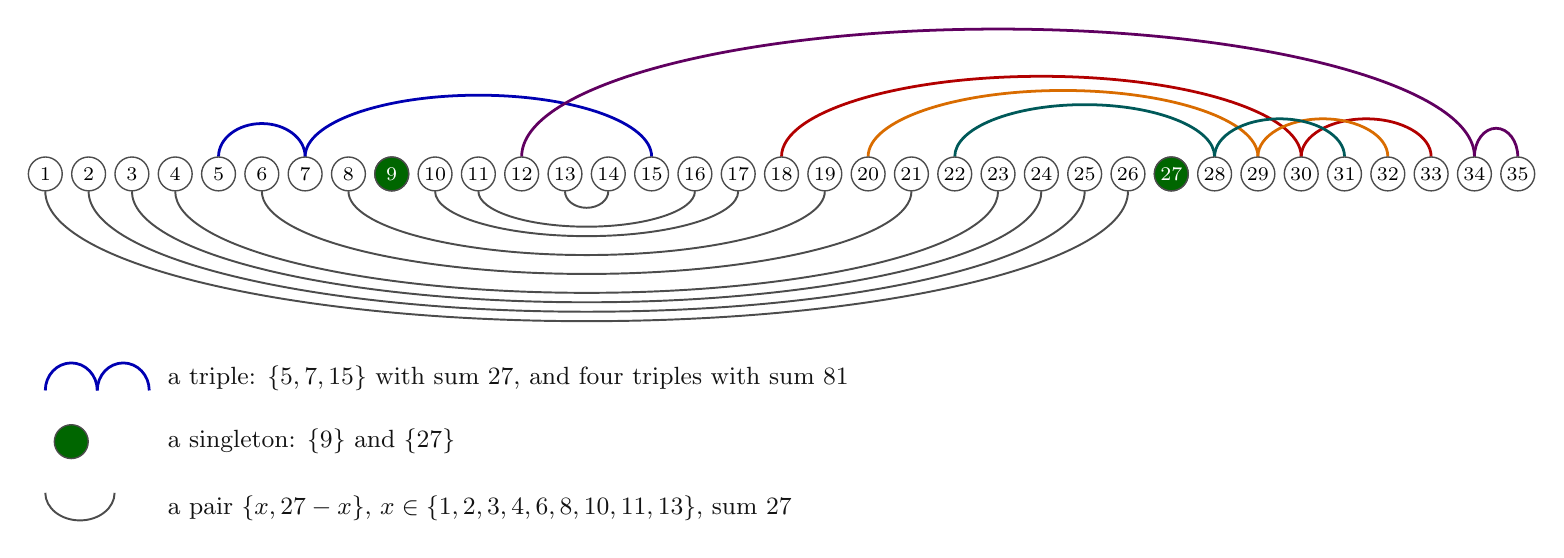
\begin{tikzpicture}[
  x=0.55cm,
  note/.style={font=\small,gray!15!black,align=left,anchor=west},
  dot/.style={circle,draw=black!70,fill=white,line width=0.5pt,inner sep=0pt,minimum size=4.3mm,font=\scriptsize}]
  % pairs {x, 27-x} below the line
  \foreach \x in {1,2,3,4,6,8,10,11,13} {
    \pgfmathsetmacro{\r}{(27-2*\x)/2}
    \draw[gray!60!black,line width=0.7pt] (\x,-0.22) arc[start angle=180,end angle=360,x radius=\r,y radius={0.12*\r+0.15}];
  }
  % triples above the line: arcs a-b and b-c, one colour each
  \foreach \a/\b/\c/\col in {5/7/15/blue!70!black, 18/30/33/red!70!black, 20/29/32/orange!85!black,
                             22/28/31/teal!70!black, 12/34/35/violet!75!black} {
    \pgfmathsetmacro{\ra}{(\b-\a)/2}
    \pgfmathsetmacro{\rb}{(\c-\b)/2}
    \draw[\col,line width=1pt] (\a,0.22) arc[start angle=180,end angle=0,x radius=\ra,y radius={0.12*\ra+0.3}];
    \draw[\col,line width=1pt] (\b,0.22) arc[start angle=180,end angle=0,x radius=\rb,y radius={0.12*\rb+0.3}];
  }
  \foreach \x in {1,...,35} { \node[dot] at (\x,0) {$\x$}; }
  \foreach \x in {9,27} { \node[dot,fill=green!40!black,text=white] at (\x,0) {$\x$}; }
  % legend
  \draw[blue!70!black,line width=1pt] (1,-2.75) arc[start angle=180,end angle=0,x radius=0.6,y radius=0.35];
  \draw[blue!70!black,line width=1pt] (2.2,-2.75) arc[start angle=180,end angle=0,x radius=0.6,y radius=0.35];
  \node[note] at (3.6,-2.6) {a triple: $\{5,7,15\}$ with sum $27$, and four triples with sum $81$};
  \node[dot,fill=green!40!black] at (1.6,-3.4) {};
  \node[note] at (3.6,-3.4) {a singleton: $\{9\}$ and $\{27\}$};
  \draw[gray!60!black,line width=0.7pt] (1,-4.05) arc[start angle=180,end angle=360,x radius=0.8,y radius=0.35];
  \node[note] at (3.6,-4.25) {a pair $\{x,27-x\}$, $x\in\{1,2,3,4,6,8,10,11,13\}$, sum $27$};
\end{tikzpicture}
\end{document}
